% !TEX root = WWW.tex
\begin{figure*}[!ht]
\centering
\subfloat[\small \textsc{google}]{
    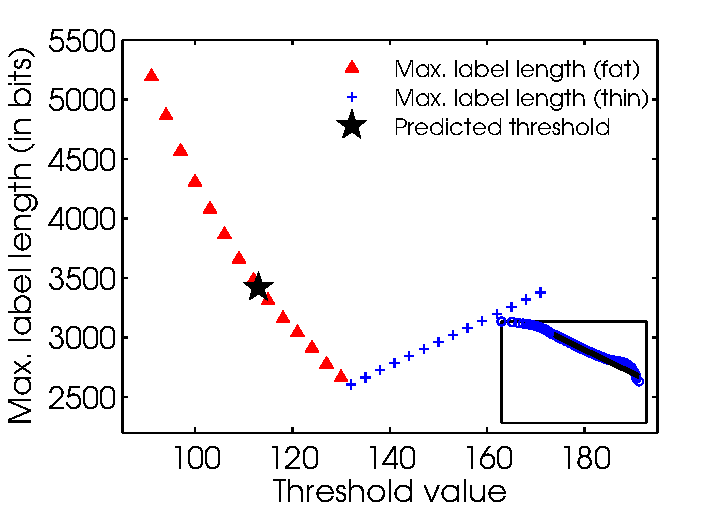
\includegraphics[width=0.32\textwidth]{Figures/web-google-revised.pdf}
}
\subfloat[\small \textsc{YouTube}]{
    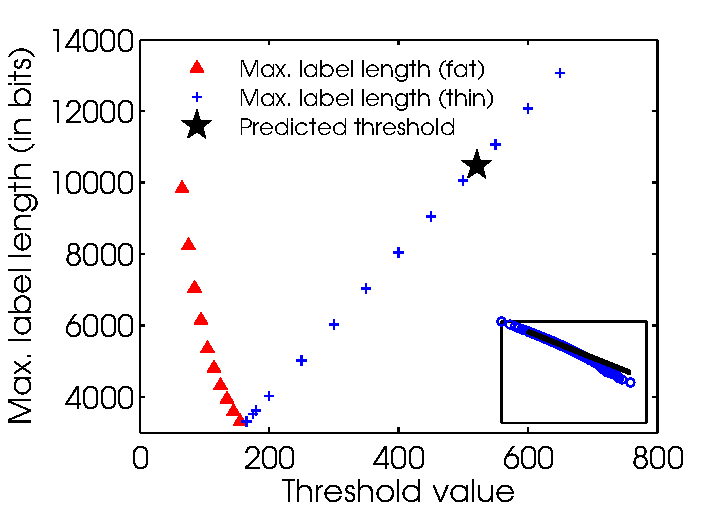
\includegraphics[width=0.32\textwidth]{Figures/web-youtube-revised.pdf}
}%
\subfloat[\small \textsc{Wikitalk}]{
    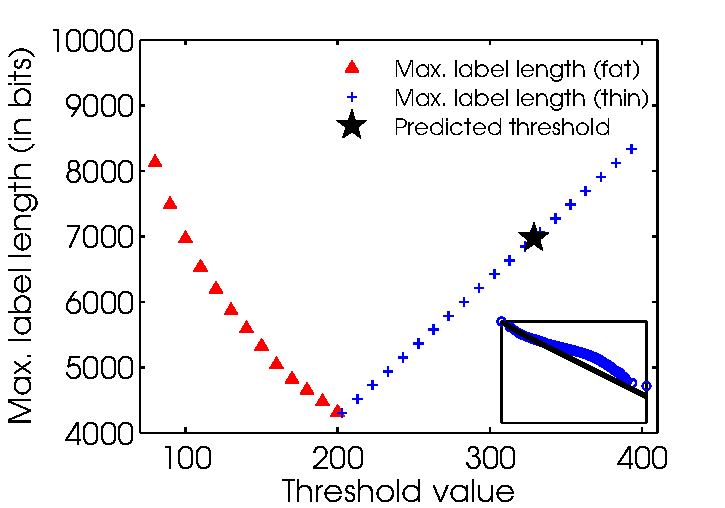
\includegraphics[width=0.32\textwidth]{Figures/web-wikitalk-revised.pdf}
}%
\caption{Predicted and empirical thresholds for the \textsc{google}, \textsc{youtube} and \textsc{wikitalk}  data sets. The inset show the MLE fitted power-law, using the method of Clauset et al.\ \cite{clauset2009power}, where data points are blue circles and the power-law is shown as a black solid. The exponents of the power-laws are shown in Table \ref{t:data sets}.}%
\label{f:bla2}%
\end{figure*}